\chapter{Background}


%===================================================================================================%
\section{Introduction}
%===================================================================================================%

"Reviews of research literature are conducted for a variety of purposes. They include
providing a theoretical background for subsequent research; learning the breadth of research on a
topic of interest; or answering practical questions by understanding what existing research has to
say on the matter. As such, research reviews are most often published as the introductory section
of an article reporting a specific research study, or as one of the early sections of an academic
thesis or dissertation. However, there exists another type of literature review that constitutes an
original and valuable work of research in and of itself. Rather than providing a base for the
researcher’s own endeavours, it creates a solid starting point for all other members of the
academic community interested in a particular topic. " (okoli, Schabram)\\
$\Longrightarrow$ UMFORMULIEREN
\clearpage
%===================================================================================================%
\section{Systematic Literature Review Method}\label{sec:LitRes}
%===================================================================================================%

The selection and review of research literature is a crucial step towards a holistic understanding of the current state of academic discussion. It is therefore utmost important to conduct it in a systematic and structured way to avoid misinformation or inchoate results. An early attempt to formalize research literature reviews was made by Fink in 2005: \blockquote{[it is] a systematic, explicit,
[comprehensive, (p. 17)] and reproducible method for identifying, evaluating, and synthesizing
the existing body of completed and recorded work produced by researchers, scholars, and
practitioners}\autocite{Fink2015ConductingPaper}. Since this approach is rather generic in order to fit many areas of research, Okoli and Schabram refined this methodology in 2010 and adapted it for \acf{IS} research. \\
According to Fink's definition, a proper and meticulous literature review is characterized by four important aspects. It should be \textit{systematic} in following a comprehensible methodological approach, \textit{explicit} in disclosing the way it was conducted, \textit{comprehensive} by including all relevant publications and therefore \textit{reproducible} and verifiable by others. 

\begin{figure}[ht]
    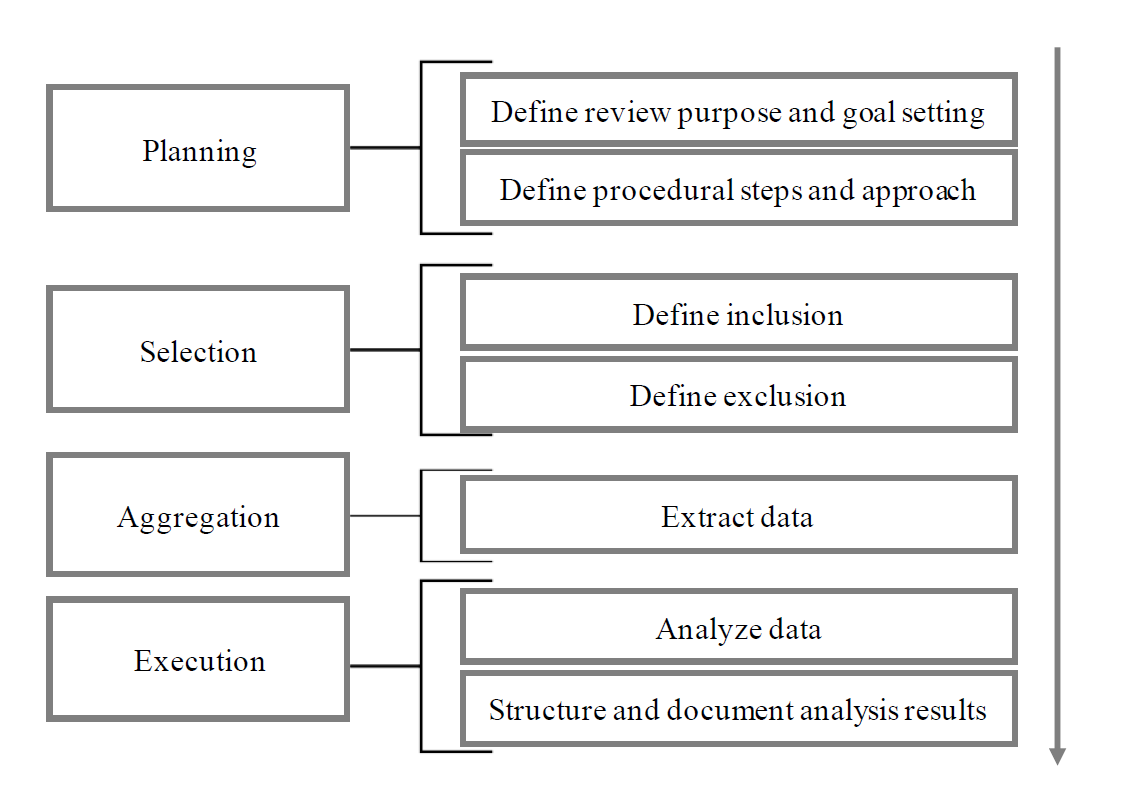
\includegraphics[width=0.8\linewidth]{images/methodology/litSearc.png}\centering
    \caption
    [Systematic Literature Review Method]
    {Systematic Literature Review Method (\cite{Okoli2010AResearch})}
    \label{fig:litSearch}
\end{figure}

As depicted in Figure \ref{fig:litSearch}, the Systematic Literature Review approach by Okoli and Schabram consists of 4 major steps: \\
\begin{enumerate}
    \item
    \textbf{Planning}\\
    First, the purpose of the research review and the goal has to be defined. This helps the review to focus on research that is truly important for his or her academic paper and conduct a consistent and traceable review. Furthermore, procedural steps should be defined. One crucial part of the planning the choice of data source. To gather relevant research to review in the following steps, numerous search engines were used to accumulate enough source material for a sufficient literature review. The engines that were used are: 
    \begin{itemize}
        \renewcommand\labelitemi{--}
        \item Google Scholar\footnote{\url{https://scholar.google.com}}
        \item Mendeley\footnote{\url{https://www.mendeley.com/research-papers/}}
        \item ScienceDirect\footnote{\url{https://www.sciencedirect.com/}}
        \item CiteSeerX\footnote{\url{http://citeseerx.ist.psu.edu/index}}
        \item GetCited\footnote{\url{https://getcited.org.cutestat.com/}}
        \item Directory of Open Access Journals\footnote{\url{https://doaj.org}}
        \item IBM Northernlight (proprietary)\footnote{\url{https://ibm.northernlight.com/}}
    \end{itemize}
    All listed engines either inherently order by \textit{relevance} or provide the user with an option to do so. The algorithmic approach on how the relevance is calculated and assessed is assumed to be correct since it is not possible for the author to verify it. Consequently, the search results are reduced to the $20$ most relevant for each search engine in the first step. Secondly, duplicates are filtered and research that was erroneously included in the results (i.e., researches that belong to different domains) is removed. The remnant results are further selected, aggregated and analyzed.
    \item
    \textbf{Selection}\\
    In this step the inclusion and exclusion of research is defined and explained. The properties to decide on which paper is excluded or included must be clearly stated in order to \textit{explicitly} disclose the approach that was taken. In this paper, relevant articles were chosen by assessing the relevance of the research title and abstract. 
    \item
    \textbf{Aggregation}\\
    After the scientific body of knowledge assessed and parts of it selected in step $1$ and $2$, the information that is relevant for the paper on hand is extracted and aggregated. This step is mainly implicit because it is merely a reduction of the selected research to a applicable amount of excerpts to directly use in the paper and results in an implicit knowledge gain by the reviewer.
    \item
    \textbf{Execution}\\
    The data is analyzed and results are presented to the reader. The main purpose of this step is to fulfill the goal defined in step $1$ and thus elevate the readers knowledge to a level that enables him or her to fully understand the authors research in the following chapters.
\end{enumerate}

The following sections will traverse these four steps in order to conduct a \textit{systematic} and \textit{consistent} research literature review. Some statements (especially step $1$ "Planning" and step $2$ "Selection") will be redundant for some domains but will be formulate nonetheless to \textit{explicitly} disclose how the results were achieved in order to maintain the \textit{reproducible} nature of this review.


%===================================================================================================%
\section{Internet of Things}
%===================================================================================================%

\begin{enumerate}
    \item
    \textbf{Planning}\\
    The purpose of this section is to give the reader a broad understanding of the industry and state of the academic research on this domain. It is not in scope to analyze different technical approaches and solutions for various use-cases but rather to enable the reader to understand the paper on hand by providing the necessary context and domain-specific terminology. Moreover, one major objective is to assess the importance of the domain and thus to confirm the significance and relevance of the research.\\
    Since the domain of \acf{IoT} is rather generic, the amount of results gathered from each search engine is expected to be vast.
    
    \item
    \textbf{Selection}\\
    For the search query \blockquote{Internet of Things}, the in Section \ref{sec:LitRes} listed engines give the following numbers of results:
    
    \begin{itemize}
        \renewcommand\labelitemi{--}
        \item Google Scholar: 2,930,000 results
        \item Mendeley: 39,826 results
        \item ScienceDirect: 58,532 results
        \item CiteSeerX: 282,506 results
        \item GetCited: 20,500 results
        \item Directory of Open Access Journals: 1,425 results
        \item IBM Northernlight (proprietary): 21,070 results
    \end{itemize}
    
    Cumulated, the queries returned 3,353,859 results from which 140 where further examined. After filtering out duplicates, 82 papers remained. Likewise, 61 papers that were either to low-level technical or not fitting to the scope in another way were excluded from the literature review. The remaining 21 results propagated to the next step, the \textit{aggregation}.
    
    \item
    \textbf{Aggregation}\\
    
    \item
    \textbf{Execution}\\
    
    
\end{enumerate}


%===================================================================================================%
\section{Event Stream Processing}
%===================================================================================================%

\begin{enumerate}
    \item
    \textbf{Planning}\\
    Similarly to the research review for \acf{IoT}, the same seven search engines were used. Likewise, the main goal is to give the reader a broad understanding over the domain and enable him to grasp the various concepts, patterns and practices in the realm of \acf{ESP}. Moreover, the purpose of this section is to explore the different limitations and challenges \acf{ESP} poses. Since it is the overall research objective to assess suitability and viability of serverless architectures for IoT Event Stream Processing, it is important to discuss and clarify the context in which the assessment will be conducted. 
    
    \item
    \textbf{Selection}\\
    For the search query \blockquote{Event Stream Processing} the following numbers of results were achieved:
    
    \begin{itemize}
        \renewcommand\labelitemi{--}
        \item Google Scholar:  1,610,000 results
        \item Mendeley: 1,726 results
        \item ScienceDirect: 207,853 results
        \item CiteSeerX: 2,460,487 results
        \item GetCited: 25 results
        \item Directory of Open Access Journals: 46 results
        \item IBM Northernlight (proprietary): 8,802  results
    \end{itemize}
    
    Cumulated, the queries returned 4,088,939 results from which 140 where further examined. After filtering out duplicates, 128 papers remained. Likewise, 113 papers that were either to low-level technical or not fitting to the scope in another way were excluded from the literature review. The remaining 15 results propagated to the next step, the \textit{aggregation}. In comparison to the selection process of IoT research, it is notable that only a fraction of the results were relevant or even related to the intended research domain.
    
    \item
    \textbf{Aggregation}\\
    
    \item
    \textbf{Execution}\\
    Event Stream Processing (or shorter \textit{Stream Processing} has become one of the most common computing tasks enterprise systems face today. As defined by the Gartner Research Institute,
    \blockquote{An event stream is a sequence of event objects arranged in some order, typically by time. \acf{ESP} is any kind of computing performed on event streams.}\autocite{Schulte2017TechnologyProcessing}\\
    In other words, \acf{ESP} processes data \textit{directly} as it is produced by nodes (i.e. applications, sensors, ...). An "event" is often just defined as a "notable thing that happens".\autocite{Group2006Event-DrivenOverview} This is a very broad definition that has to be revised and adapted to the specific use-case at hand but a shared characteristic is that all events contain information, are generated as a byproduct of the occurrence of something and can be associated with a specific point in time. 
    Since many real world scenarios such as sensor measurements, financial trades, and so forth regularly result in a continuous stream of events, \acf{ESP} is often a viable architectural approach.\\
    The traditional solution for this challenge is to store the data in a database and let applications query the data as needed or as scheduled. As depicted in \ref{fig:dataRest}, the occurring events are sent from an application or sensor to an endpoint where they are stored at rest and the computation of said events has to be scheduled and managed. It is important to note that the information flow in this model centers around the data storage. First the information flows from the source to it and after that the downstream applications have to make some kind of request to it to access the information.
    
    \begin{figure}[ht]
        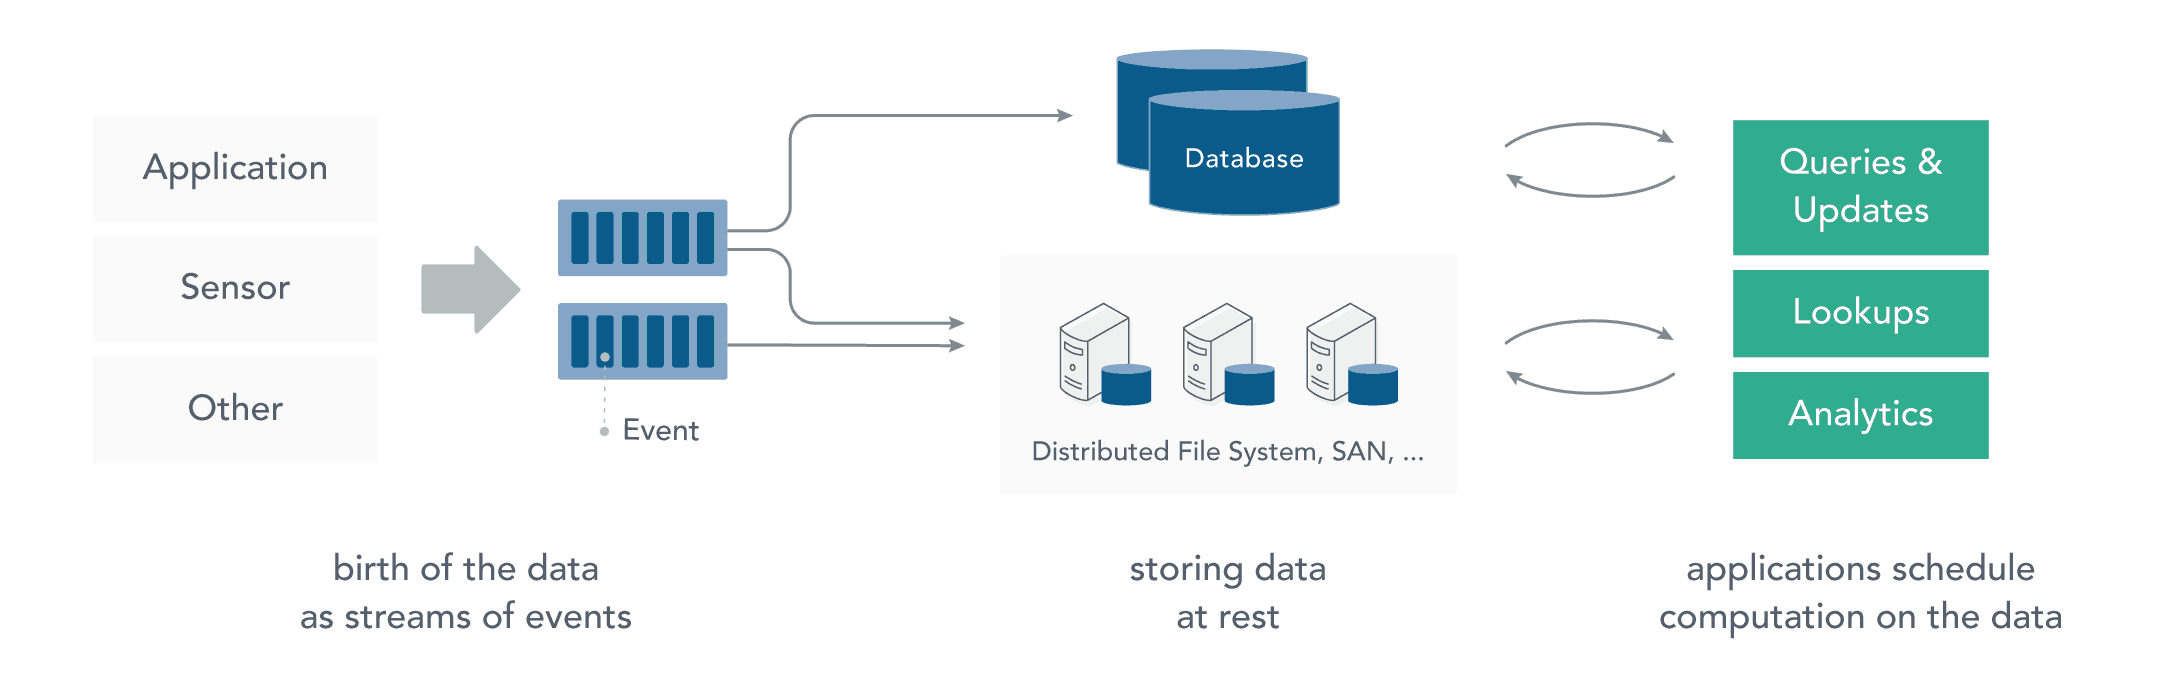
\includegraphics[width=\linewidth]{images/streaming/data_at_rest.png}\centering
        \caption
        [Data-at-Rest Architecture]
        {Data-at-Rest Architecture (\cite{dataArtisans2017WhatProcessing})}
        \label{fig:dataRest}
    \end{figure}
    
    With Stream Processing however, a continuous data flow from left to right is established. Upon receiving an event from the stream, the \acf{ESP} application performs a task based on the event. For instance, this could be a transformation of the events properties in order to match system-wide standards (e.g., unit conversation). 
    Figure \ref{fig:dataStream} shows a simplified example of this pattern. Similarly to figure \ref{fig:dataRest}, applications, sensors or other clients continuously generate events that are sent to an endpoint but instead of storing the data, it is directly processed by the assigned application. As indicated by the two arrows that lead from two streams to one single application, it is likewise possible to process multiple streams jointly and merge numerous information flows. The so-called \textit{stream processors} directly react upon receiving the events as mentioned before. 
    
    \begin{figure}[ht]
        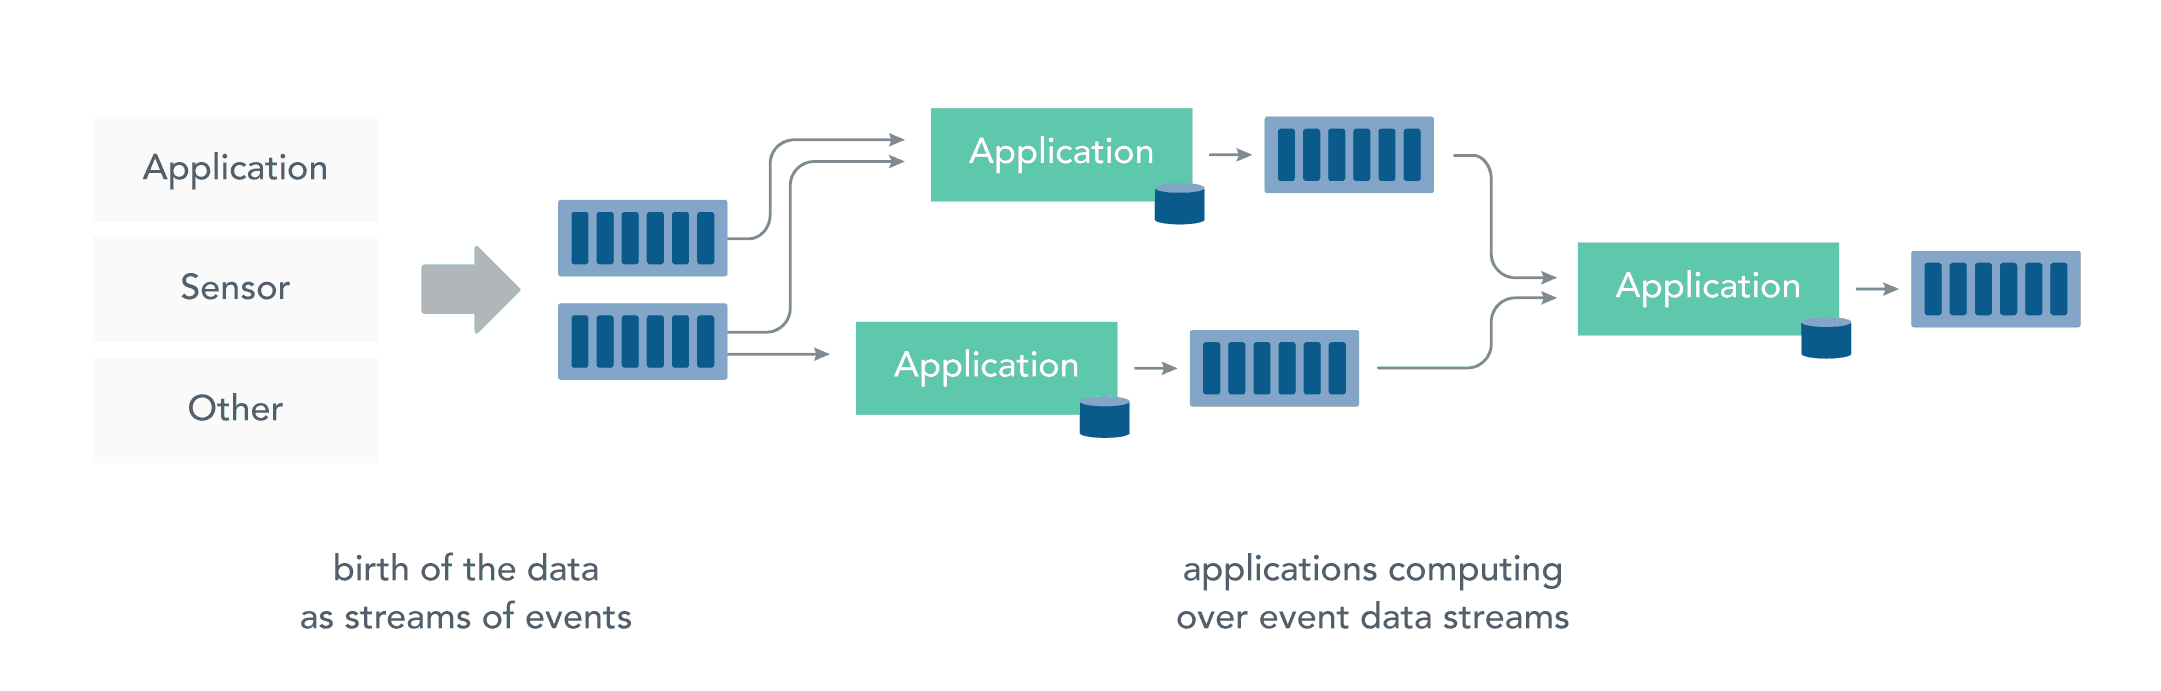
\includegraphics[width=\linewidth]{images/streaming/streming_data.png}\centering
        \caption
        [Stream Processing Architecture]
        {Stream Processing Architecture (\cite{dataArtisans2017WhatProcessing})}
        \label{fig:dataStream}
    \end{figure}
    
    This seemingly small change to the information flow has some serious implications. To begin with, \acf{ESP} resembles the natural flow of data outside the IT system much closer than scheduled computation and is therefore easier to understand and design for. Secondly, since the event is processed immediately upon being received, the application can react instantly and a lag time between the occurrence of the event, the action trigger and the action itself can be avoided which results in a near real-time processing of information. 
    
    This approach allows for a data-driven and computation-driven perspective on complex business problems that aim to provide dynamic insights and need to handle a steady input of information. 
    Due to recent trends in the industry such as IoT and Industry 4.0, the amount of data that has to be categorized, analyzed and processed skyrocketed. The data-ingress often consists of semi-structured sets and has to be transformed and handled in near real-time.\autocite{Dekate2017PredictsInfrastructure} In order to provide valuable business insights for companies and public sector players alike, this approach is likely not only a temporarily trend but rather a long lasting evolution of the way data-centric enterprise systems are being designed. Moreover, a recent Gartner report predicts that the market for \acf{ESP} solutions will grow by 15\% year over year from 2017 to 2022 (compound annual growth rate).\autocite{Heudecker2017MarketProcessing} \\
    Many companies such as Netflix\footnote{\url{https://aws.amazon.com/solutions/case-studies/netflix-kinesis-streams/}} or Uber\footnote{\url{https://flink.apache.org/poweredby}} adopted stream-processing patterns in combination with serverless computing to take on challenges that demand highly scale able and performant systems. 
    This approach is particularly favourable for companies that deliver IoT solutions such as Toyota\footnote{\url{https://aws.amazon.com/solutions/case-studies/toyota-tsusho/}} or Quest\footnote{\url{https://customers.microsoft.com/en-us/story/quest}}.
    
\end{enumerate}


%===================================================================================================%
\section{IoT Event Stream Processing}
%===================================================================================================%

\begin{enumerate}
    \item
    \textbf{Planning}\\
    Since the background of this research is \blockquote{IoT Event Stream Processing}, the connection of both academic fields, IoT and Event Stream Processing, has to be discussed and put in context. Because the basic collection of research has been done in the two previous sections it is not necessary to gather another sample of academic papers and hence the act of querying search engines can be omitted. Instead, papers from the preceding reviews that contain linking information for both IoT and ESP will be presented to connect both domains.
    
    \item
    \textbf{Selection}\\
    
    \item
    \textbf{Aggregation}\\
    
    \item
    \textbf{Execution}\\
    
\end{enumerate}


%===================================================================================================%
\section{Data Consumer Architecture Patterns}
%===================================================================================================%

\begin{enumerate}
    \item
    \textbf{Planning}\\
    Since the topic of Data Consumer Architecture Patterns is the most crucial component 
    
    \item
    \textbf{Selection}\\
    
    \item
    \textbf{Aggregation}\\
    
    \item
    \textbf{Execution}\\
    
\end{enumerate}

%***************%
\subsection{Containerized Application}
%***************%

\begin{figure}[ht]
    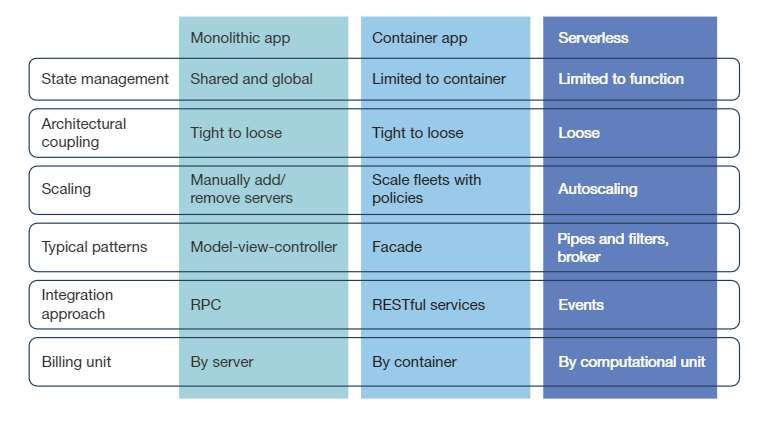
\includegraphics[width=\linewidth]{images/serverless/demyst.png}\centering
    \caption
    ["Serverless" compared to traditional approaches]
    {"Serverless" compared to traditional approaches (\cite{Hammond2018DemystifyingComputing})}
    \label{fig:slessCompared}
\end{figure}

Problems:
\begin{enumerate}
    \item tightly coupled
    \item hard to scale
    \item hard to apply eventD models
    \item Integration (ESB)  Servicefull
    \item billing unit not tied to business logic
\end{enumerate}


%***************%
\subsection{Serverless}
%***************%

"Serverless" is \textbf{the} new hype technology and is estimated to grow from USD 1.88 billion in 2016 to USD 7.72 billion by 2021, at a Compound Annual Growth Rate (CAGR) of 32.7\% according to "Markets and Research".\autocite{2017Function-as-a-Service2021} 

Traditional approaches such as monolithic on-premise systems and even \acf{PaaS} based solutions or container clusters can be an option but have their own advantages and caveats. As shown in Figure \ref{fig:slessCompared}
(page \pageref{fig:slessCompared}), Hammond and Ryner identify six major categories to characterize architectural approaches.\\
\textbf{State Management} is one of the areas where \textit{monolithic apps} have the most obvious advantage. The state is shared and global which reduces the required state management to a bare minimum. Since \textit{monolithic apps} are defined as one single system that offers many services using different interfaces that share the same global state. \autocite{Villamizar2015EvaluatingCloud} The management of this state is therefore not particularly complex and can be done inside of the system. For availability reasons, it might be a good idea to store the state redundantly but this is out of scope for the thesis and does not change the fact that the state of a \textit{monolithic app} is shared and global.\\
For a \textit{container app} on the other hand, state management is normally limited to the container. Since one of the main design principles of containerization is to confine the system within the boundaries of the container, it is possible to maintain a global shared state within the container itself but not to share it between all system services. If one container dies (e.g., reboot, failure, ...), it's state dies with it. Concepts like state-providers act as an external source of truth that can transfer and preserve state but often add complexity to the system and need to be implemented.\autocite{Ling2004SessionState}\\
Similarly, state management in \textit{serverless applications} can be complex due to the confined nature of its code. Since the application is spun up on invocation and only lives on for the computation time it is not possible to maintain state throughout different function invocations.

"Serverless" computing aims to solve those problems.\autocite{Roberts2016ServerlessArchitectures}


%===================================================================================================%
\section{Summary}
%===================================================================================================%